\section{Technical Aspects and User guide}
The data library is stored as a collection of Advanced Scientific Data Format (ASDF) files \cite{greenfield2015a}. ASDF is a new interchange format for scientific data developed by the Space Telescope Science Institute primarly for astronomy and is still in active development. This format was chosen due it's hierarchical and human-readable metadata format and it's native Python data types. This ensures the library remains usable despite version changes of computational tools used as well as easily storing the source of the data. The official data library and it's associated tools is maintained by Copenhagen Atomics as an open source project on GitHub.\\ \newline
Following the data library is a Parser which allows users to add custom data into the data library while keeping the format correct which makes it easy for contributors to expand the data library. A secondary API script is also included which handles basic data processing of the library for researchers. Both of these tools are written in Python 3.6 and some basic knowledge of the language is required to utilize the tools. To aid with some specific functions some packages not included in the Python base library are used, shown in table \ref{tab:dependencies}. The most important feature of API is to easily extract all data that matches a requested physical property and component mixture and organizing the data into arrays that allow for further data analysis. A secondary feature of the API is to fit the data to a variety of basis function if applicable and build a mathematical model around the data.\\

The API currently uses Regression Kriging model as the surrogate model to fit and predict data. Kriging model has been used extensively in engineering to model and understand sparse data\cite{forrester2008a} which makes it a strong tool for the data library where we expect sparse datasets when it comes to different mixing ratios of the salts. The mathematical description of Kriging models is illustrated by Jones et al\cite{Jones2001}. Ordinary Kriging is designed as an exact interpolation technique which may lead to high oscillating behaviour when dealing with datasets that are expected to be noisy. The problem is addressed by using the augmentation to Kriging where a regression component is added\cite{HENGL20071301}. These models are created using the Python package pyKriging, which is an open source package maintained by Paulson and Ragkousis\cite{paulson_2015_21389}.

\begin{table}[htp]
    \centering
    \caption{List of 3rd party Python dependencies}
    \begin{tabular}{c | c}
    \hline
    Name     &  Function  \\ \hline
    asdf     &  Handles creation and manipulaton of ASDF files \\
    openpyxl &  For extracting data from Excel Files \\
    numpy &  Numerical array object \\
    matplotlib & Creating Figures \\
    scipy & For the optimize functionality to fit regression parameters \\
    pyKriging & For training of a Kriging Model \\
    \hline
    \end{tabular}
    \label{tab:dependencies}
\end{table}
To fully utilize all aspects of the program the dependencies listed in Table \ref{tab:dependencies} must be installed, access to Microsoft Excel is required as well in the current version. \\
Each file in the library contains the experimental results of a journal article, book etc. converted into a tree like structure which makes it easy for a python script to navigate and extract raw data for further data processing. The experimental data is saved as a data set, where each data set contains temperature readings and the measurements of a single physical property of a salt mixture. It will also contain any optional information supplied by the authors such as regression, errors etc. The raw data itself can be extracted using Python's numpy package as asdf by default compresses the data for better efficiency. Each file also contains a metadata tree which contains creation and update times of the file itself as well as reference to the data written in a bibTeX format.

\begin{figure}[h]
\centering
\begin{minipage}{0.5\textwidth}
  \centering
  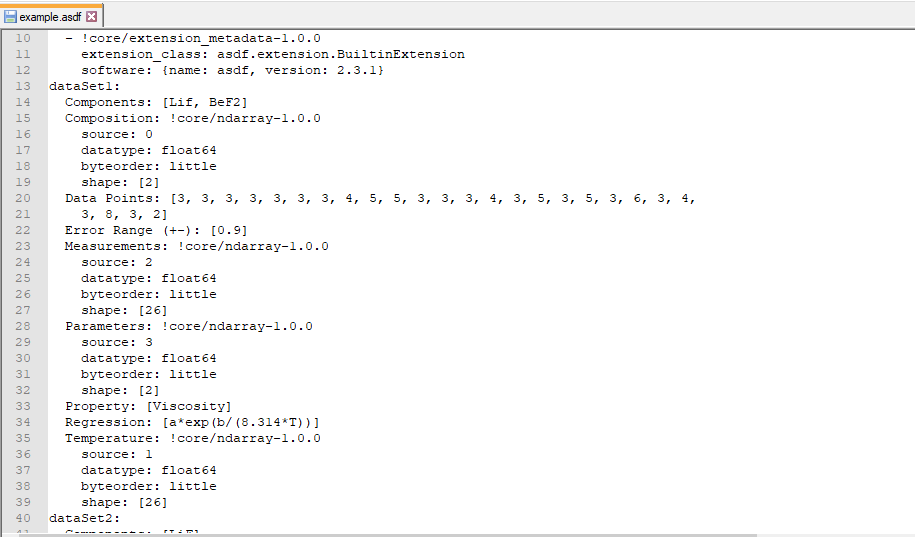
\includegraphics[width=\linewidth]{msdf/figures/asdfEx1.PNG}
\end{minipage}%
\begin{minipage}{0.5\textwidth}
  \centering
  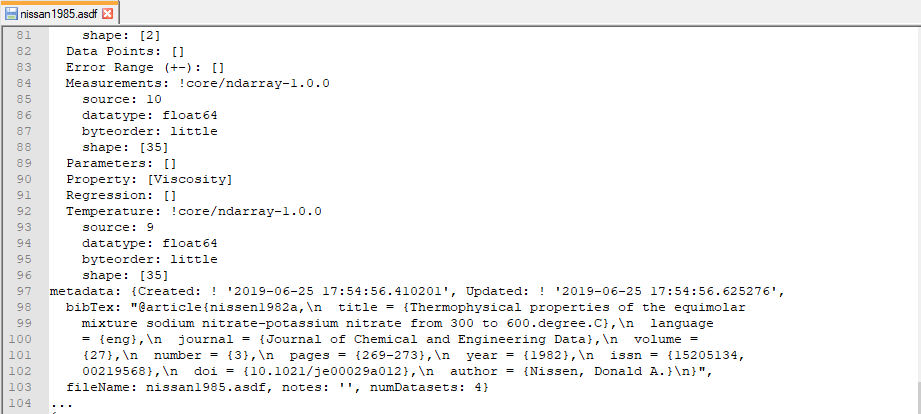
\includegraphics[width=\linewidth]{msdf/figures/asdfEx2.PNG}
\end{minipage}
\caption{Example of an asdf file structure, with a) depicting a dataset structure and b) depicting the metadata}
\label{fig:asdfExample}
\end{figure}

\subsection{Introduction to Parser}
The parser source code is contained in the file \textit{ooASDF.py} located in the \textit{Director} folder, it is written to scan excel file containing experimental data points as well as text files containing citation information and create asdf file with the proper tree structure and syntax as shown in figure \ref{fig:asdfExample}. Before using the parser, it is necessary to prepare two files, an Excel file containing the raw data and optional information in a specific structure and a text file containing reference information in a bibTeX format. An example Excel file is shown in figure \ref{fig:excelEx}. Note that each asdf file is reserved for a single source, so if a single report or book contains multiple data sets for multiple salts or properties it is necessary separate them into new identical  Excel sheets, the Parser will scan all Excel sheets and treat them all equally. It is important the data input for the excel files matches the units showcased in Table \ref{tab:unitStandards}. The information with red lettering is a requirement to fill out, but anything in green is optional and any additional information the user wants to convert can be added by going down the rows.

\begin{figure}[h]
    \centering
    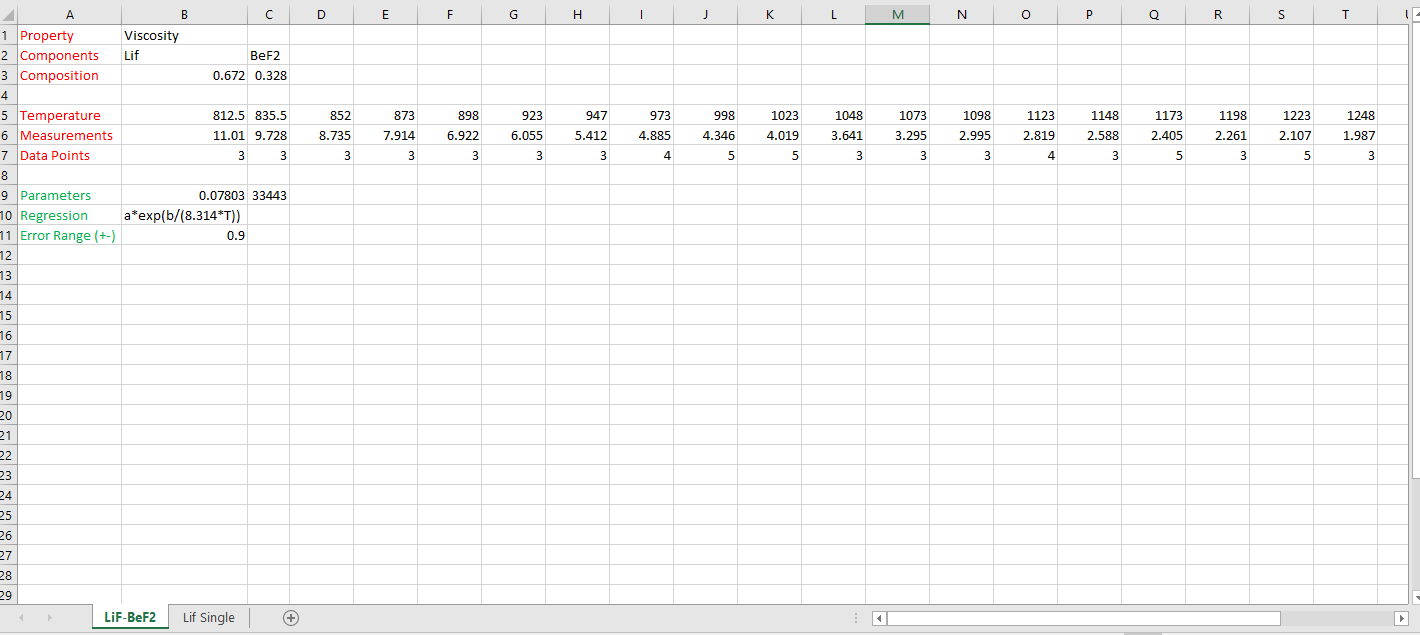
\includegraphics[width = 0.7\textwidth]{msdf/figures/excelEx.PNG}
    \caption{Example Excel file with correct structure and syntax}
    \label{fig:excelEx}
\end{figure}

\begin{table}[h]
    \centering
    \caption{List of physical properties currently in the database with expected associated unit and basis function to regress Temperature dependent data to parameters $a$,$b$ and $c$.}
    \begin{tabular}{c|c|c}
    \hline
    Property     & Unit & Fitting Function  \\ \hline
    Temperature     & \textdegree{}C  & N/A\\
    Density & $g/cm^3$ & $a+bT$\\ 
    Viscosity & $Pa \, s$ & $a*exp(b/(8.314T))$\\
    Surface Tension & $dyn/cm$ & $a+bT$\\
    Electrical Conductance & $1/(ohm\, cm)$ & $a + bT + cT^2$ \\
    Heat Capacity & $cal/(K\,mol)$ & $a + bT + cT^{-2}$ \\
    Vapor Pressure & $mmHg$ & $10^{a + b/T}$ \\
    Thermal Conductivity & $10^4* \, cal/(cm\,sec\,K)$ & $a + bT$\\
    \hline
    \end{tabular}
    \label{tab:unitStandards}
\end{table}

The reference file can simply be a Text File that contains reference information in bib format as raw text. One of the primary features of the project is the ability to track all the experimental data, meaning this is a requirement when creating new files. If the reference information is missing the program will throw an error.
 These two Input files should then be placed in the \textit{Input Files} folder as seen in figure \ref{fig:inputStruct} before running the program. Afterwards the Excel and reference text files will be stored in the \textit{Converted Files} folder\\

\begin{figure}[h]
    \centering
    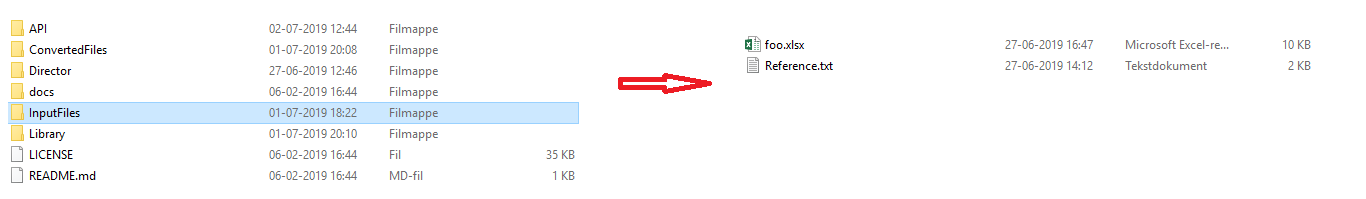
\includegraphics[width = 0.7\textwidth]{msdf/figures/input.png}
    \caption{Showcasing where to put Excel and Reference Files}
    \label{fig:inputStruct}
\end{figure}

Using the program can be done either by typing in the commands at the bottom of \textit{ooASDF.py} as shown in figure \ref{fig:ooASDFtypeLocation} file or by importing the ooASDF class from \textit{ooASDF.py}, It is important not to change the working directory when using the program and keep it the \textit{Director} folder to ensure that the manipulated files end in \textit{Library} folder. Below is a table of the functions for the program and a couple of example usages.

\begin{figure}[h]
    \centering
    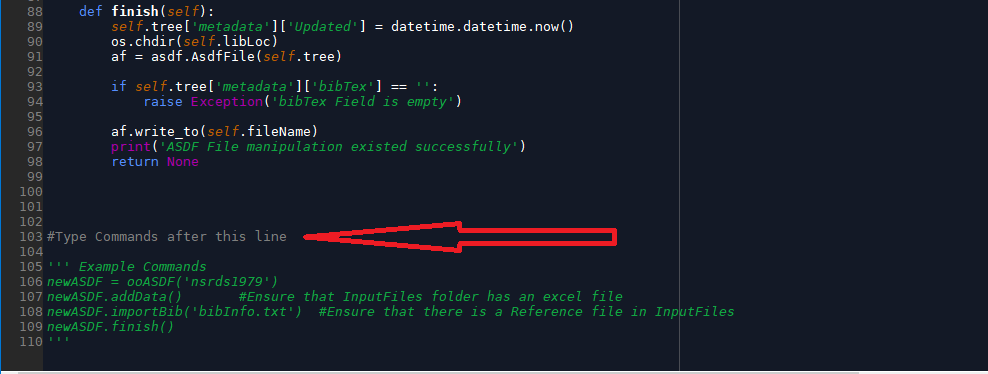
\includegraphics[width = 0.7\textwidth]{msdf/figures/ooASDFwhereToType.PNG}
    \caption{Snapshot of the program source code showcasing where to write new commands}
    \label{fig:ooASDFtypeLocation}
\end{figure}

\begin{table}[h]
    \centering
    \caption{List of ooASDF methods}
    \begin{adjustbox}{width=1\textwidth}
    \begin{tabular}{c|c}
    \hline
    Method    & Usage  \\ \hline
    ooASDF(fileName) & Constructor, opens up the specified file or creates one if it doesn't exist \\
    .addData() & Scrapes the Excel File and collects the data \\
    .importBib(fileName) & Imports the contents of fileName into a string to use as reference information \\
    .finish() & Writes the collected data into an asdf file\\
    \hline
    \end{tabular}
    \end{adjustbox}
    \label{tab:ooASDFmethods}
\end{table}


\subsubsection{Adding data to existing file}
If a file already exists in the library but data is missing and needs to be added, the reference bib file is not necessary. Filling up the Excel file akin to figure \ref{fig:excelEx} and putting it in the \textit{Input Files} should be done first. Then use the following three commands to add the data.
\begin{verbatim}
    asdfFile = ooASDF('existingFile')
    asdfFile.addData()
    asdfFile.finish()
\end{verbatim}
The first line opens up an existing datafile, the second line scans all the Excel sheets and adds the data to it and the third line updates the datafile with the scraped information and updates the metadata.

\subsubsection{Creating new file}
Creating a new datafile is very similar as updating an existing one, except now it is necessary to include the reference information along with the Excel file in \textit{Input Files}

\begin{verbatim}
    newFile = ooASDF('newFile')
    newFile.addData()
    newFile.importBib('bibInfo.txt')
    newFile.finish()
\end{verbatim}
This follows a very similar workflow as for adding data except now the first line creates the new datafile with the specified file name and the third line scans in the reference information and adds it to the metadata. Trying to build a new datafile without using .importBib() method will result in an error due to missing source.

\subsection{Introduction to API}
The API source file is \textit{api.py} located in \textit{API} folder. This part of the program handles all data extraction from the molten salt data library while also containing some data processing features such as regression, model fitting and visualization. Using the api to do dataprocessing is simply importing the \textit{api} class or use the \textit{api.py} source file similar to how to use the Parser and simply ask for a physical property and a salt mixture. Optionally it is possible to extract specific mixing ratios of the molten salt. After running the parser a new \textit{output.xlsx} file is created which contains the filtered information found in the data library as well as regression information if applicable. Table 

\begin{table}[h]
    \centering
    \caption{List of API functions and methods}
    \begin{adjustbox}{width=1\textwidth}
    \begin{tabular}{c|c}
    \hline
    Method    & Usage  \\ \hline
    API(Property,Salt List, \textit{Composition}) & Constructor to set up the object, the \textit{Composition} argument is optinal \\
    .scanLibrary() & Scans the entire library for matching salt mixture and physical property \\
    .organizeData() & Organizes the data into X and Y arrays ready for data analysis \\
    .regressData() & Regresses data of single mixtures to a basis function in table \ref{tab:unitStandards}\\
    .buildModel() & Builds a mathematical model of the data, currently Regression Kriging model \\
    .makePlot() & Visualizes the data in graphical format \\
    .printExcelReport() & Creates the \textit{output.xlsx} file with all the gathered data \\
    .initializeData() & Combines scanLibary(), organizeData() and printExcelReport() methods for pure data extraction\\
    .intializeFull() & Combination of all above function for full data analysis of given salt mixture \\
    \hline
    \end{tabular}
    \end{adjustbox}
    \label{tab:apiMethods}
\end{table}

Below are some example usages on the program to extract relevant information from the library

\subsubsection{Extracting raw viscosity data of $CaCl_2$}
Simply extracting raw data from library containing only viscosity data of $CaCl_2$ can be done in two commands
\begin{verbatim}
    CaCl2Dat = API('viscosity',['CaCl2'])
    CaCl2Dat.initializeData()
\end{verbatim}
Where first command creates the Python object and second command combines the API features of scanning, organizing and output into an excel file. This will result in an excel file depicted in

\begin{figure}[h]
\centering
\begin{minipage}{0.5\textwidth}
  \centering
  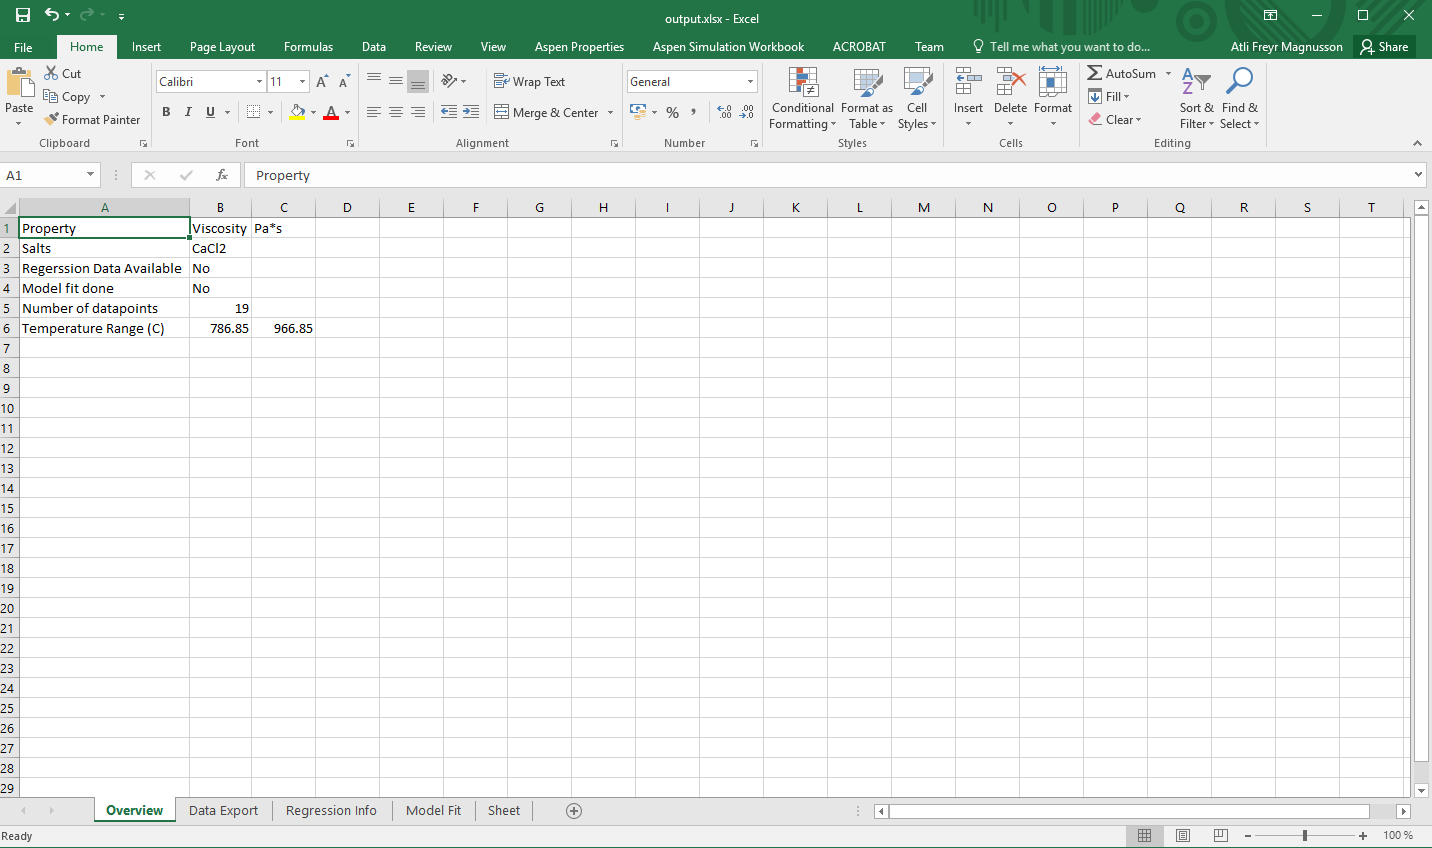
\includegraphics[width=\linewidth]{msdf/figures/caclOverview.PNG}
\end{minipage}%
\begin{minipage}{0.5\textwidth}
  \centering
  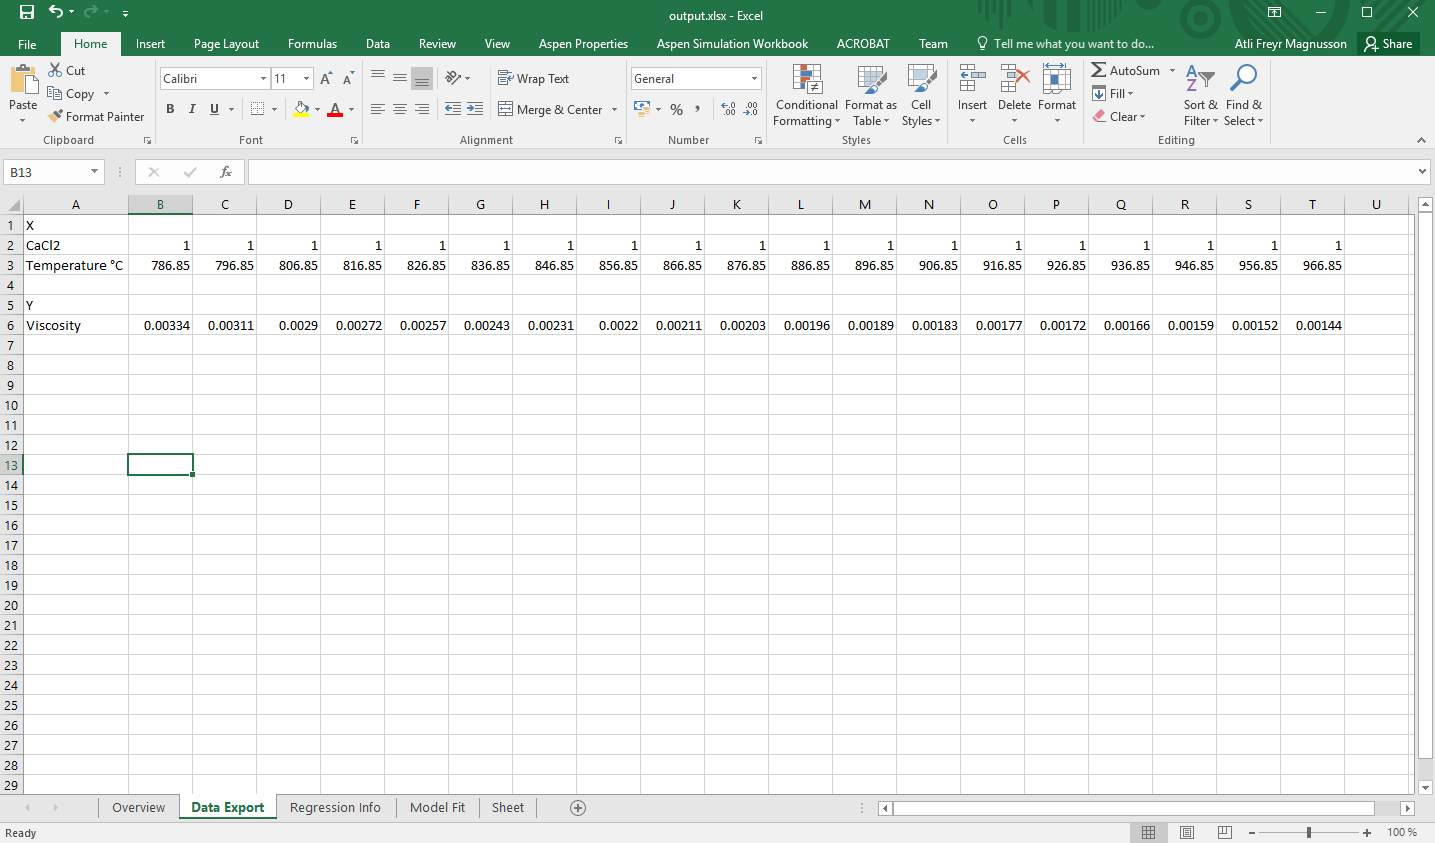
\includegraphics[width=\linewidth]{msdf/figures/caclExport.PNG}
\end{minipage}
\caption{Example Excel output when asking for viscosity data of molten $CaCl_2$.}
\label{fig:caclExcel}
\end{figure}

\subsubsection{Full regression and model building of $CaCl_2$ viscosity data}
To utilize all the data processing features implemented so far two commands are needed, similar to above commands except replace initializeData() with intializeFull().

\begin{verbatim}
    CaCl2Obj = API('viscosity',['CaCl2'])
    CaCl2Obj.initializeFull()
\end{verbatim}
This also results in the Excel information depicted in figure \ref{fig:caclExcel}, but now the Regression Info and Model Fit sheets also contain information shown in figure \ref{fig:caclFits}. The Regression Info contains the basis function used, the fitted parameters and an illustration of the regression. The Model Fit only contains an illustration of the Kriging model due to it's complexity. 


\begin{figure}[h]
\centering
\begin{minipage}{0.5\textwidth}
  \centering
  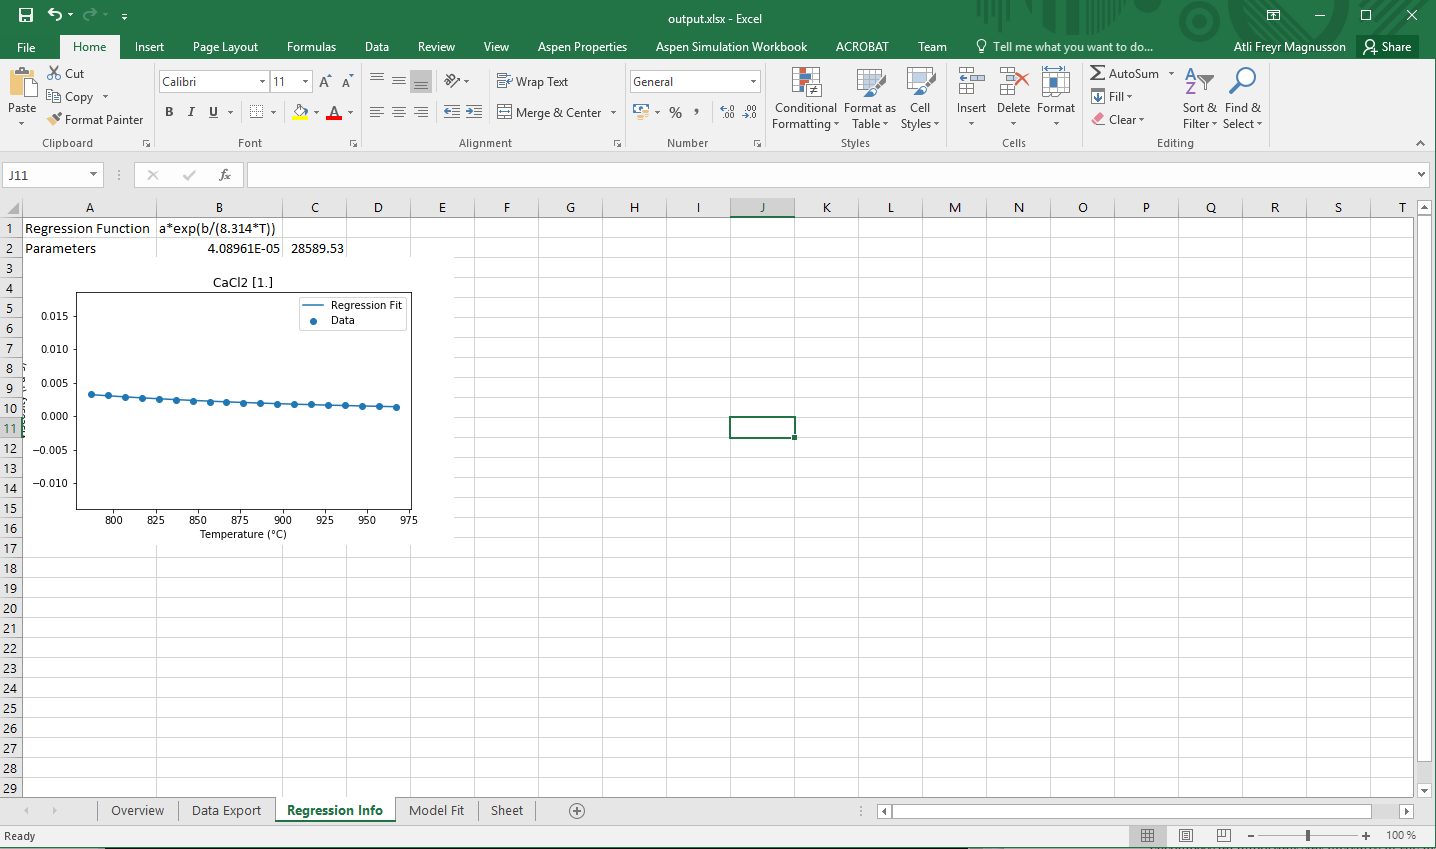
\includegraphics[width=\linewidth]{msdf/figures/caclRegression.PNG}
\end{minipage}%
\begin{minipage}{0.5\textwidth}
  \centering
  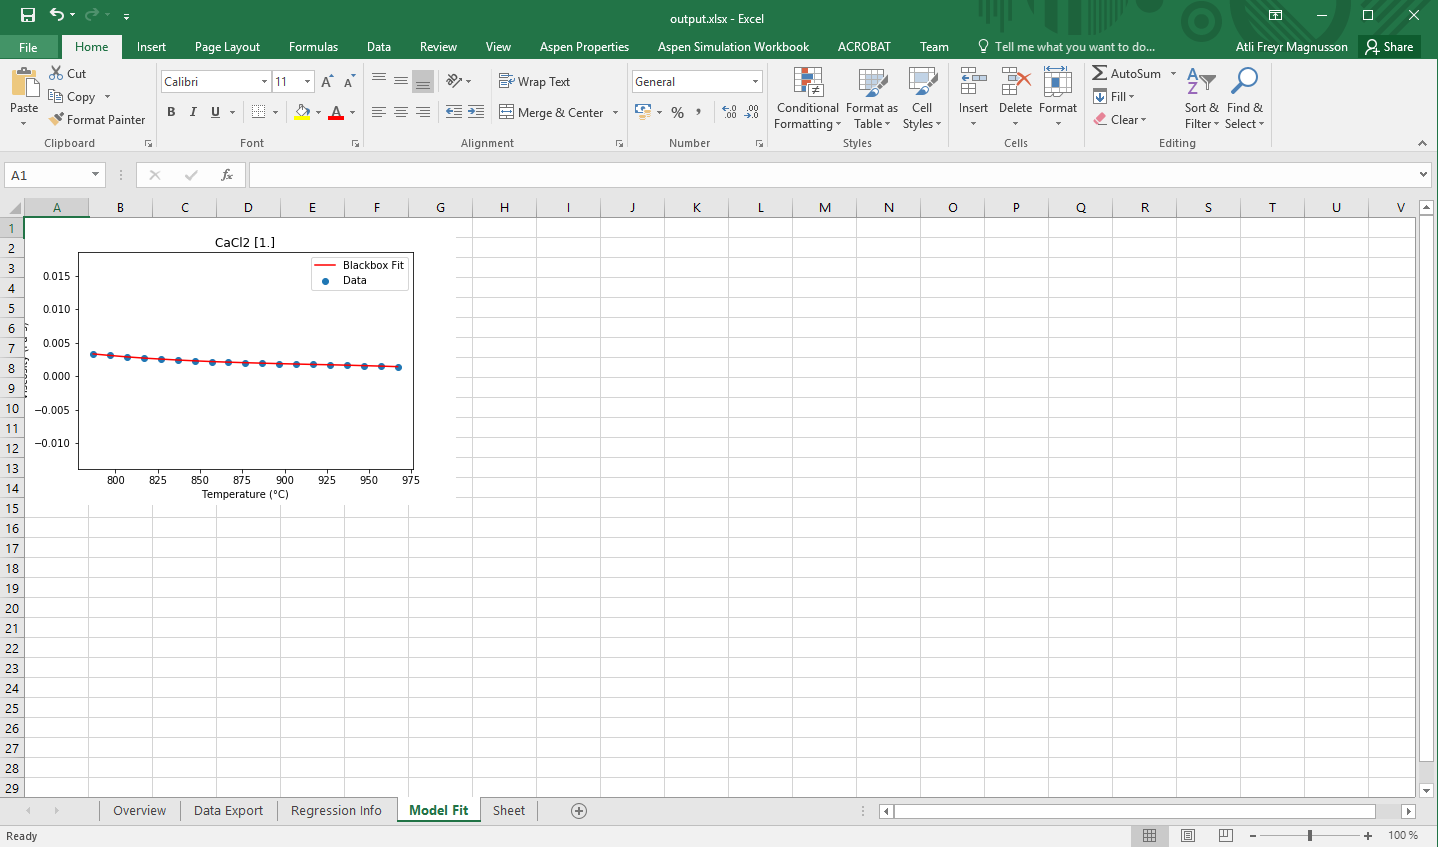
\includegraphics[width=\linewidth]{msdf/figures/caclBlackBox.PNG}
\end{minipage}
\caption{Results of Regression and Model fitting of $CaCl_2$ viscosity data}
\label{fig:caclFits}
\end{figure}


The Regression Kriging model can still be used to predict new data points. The regression model is stored in the variable \textit{fitModel} in the Python object and has the .predict() method which accepts a Temperature coordinate and outputs a prediction. A full command example:
\begin{verbatim}
    CaCl2Dat.fitModel.predict([862.52])
    >>0.002147126842301393
\end{verbatim}

\subsubsection{Analysis of a single $LiCl-KCl$ mixture with a molar ratio 20\% molar percentage of $LiCl$}
When dealing with a salt mixture that in the library holds temperature dependent data for multiple mixing ratios like for the $LiCl-KCl$ system, it is possible to specify the mixing ratio as desired with an optional mixing ratio input to the API() command.

\begin{verbatim}
    binaryMixture = API('density',['LiCl','KCl'],[20,80])
    binaryMixture.initializeFull()
\end{verbatim}
This will result in a similar \textit{output.xlsx} as for a single salt system depicted in figures \ref{fig:caclExcel} and \ref{fig:caclFits}. The \textit{fitModel} feature works under the same condition as above. Since only temperature dependence is analysed the visualization is a 2D plot exploring temperature dependence as shown in figure \ref{fig:Licl20}.

\begin{figure}[h]
\centering
\begin{minipage}{0.5\textwidth}
  \centering
  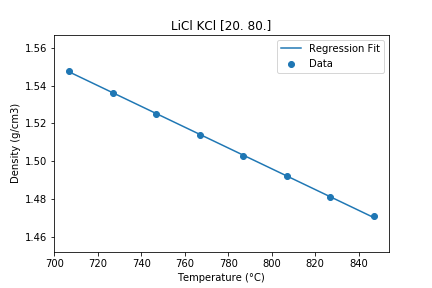
\includegraphics[width=\linewidth]{msdf/figures/LiCl20Reg.png}
\end{minipage}%
\begin{minipage}{0.5\textwidth}
  \centering
  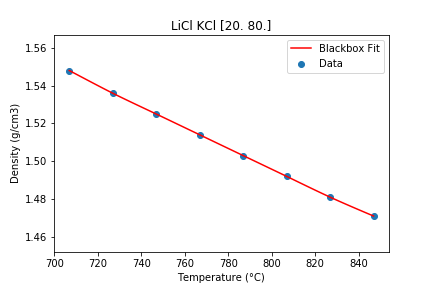
\includegraphics[width=\linewidth]{msdf/figures/LiCl20Bl.png}
\end{minipage}
\caption{Example output when asking for density analysis of 20-80 Mixture of $LiCl-KCl$}
\label{fig:Licl20}
\end{figure}

\subsubsection{Modelling density of $LiCl-KCl$ system for different mixing ratios}
Alternatively it is possible to extract the data and get a model fit for the entire system at all mixing ratios. In this case there is no regression done as now the program also analyses effect of mixing and currently we lack a basis function that accounts for both temperature and mixing dependencies. Thus only fitting done is the Regression Kriging model. To run this analysis for a salt mixture that contains data for multiple mixing ratios simply skip the mixing ratio parameter in the API() call.

\begin{verbatim}
    binaryMixture = API('density',['LiCl','KCl'])
    binaryMixture.initializeFull()
\end{verbatim}
Since this is a binary mixture we can depict the fit model as a 3D surface plot depicted in figure \ref{fig:liclsurfade}. This is done automatically for all binary mixtures, however no illustration is made for ternary or higher dimensional mixtures.

\begin{figure}[h]
    \centering
    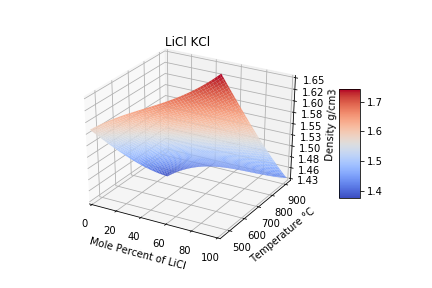
\includegraphics[width = 0.7\textwidth]{msdf/figures/LiClSurface.png}
    \caption{Surface plot of $LiCl-KCl$ Regression Kriging model predicting Density}
    \label{fig:liclsurfade}
\end{figure}

Using the fitted model is done with a similar syntax as for a single salt case but this case a mixing coordinate also has to be passed into the .predict() method. For a binary case simply put the mole percentage of the first case and then Temperature in Celsius. 

\begin{verbatim}
    binaryMixture.fitModel.predict([62.3,752.4])
    >>1.5096203630922684
\end{verbatim}
If the mixture contains more salts, then to use the prediction function it is necessary to pass the entire mixing coordinate and then supply the temperature

\begin{verbatim}
    ternaryMixture = API('viscosity',['lif','bef2','thf4'])
    ternaryMixture.initializeFull()
    ternaryMixture.fitModel.predict([0.62,0.34,0.04,895.5])
    >>0.8954644016700709
\end{verbatim}


\textit{Note}: Most salt systems currently in the library only contain a single mixture, in this case data analysis reverts to a single mixture as in 3.2.3 automatically, even if no mixing ratio was specified.\\
Example when asking for data on a $LiF-BeF_2$ mixture

\begin{verbatim}
    binaryMixture = API('density',['Lif','BeF2'])
    binaryMixture.initializeFull()
\end{verbatim}
This will results in illustrations depicted in figure \ref{fig:lifbef}.

\begin{figure}[h]
\centering
\begin{minipage}{0.5\textwidth}
  \centering
  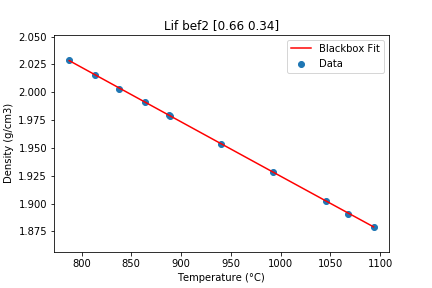
\includegraphics[width=\linewidth]{msdf/figures/lifbefRe.png}
\end{minipage}%
\begin{minipage}{0.5\textwidth}
  \centering
  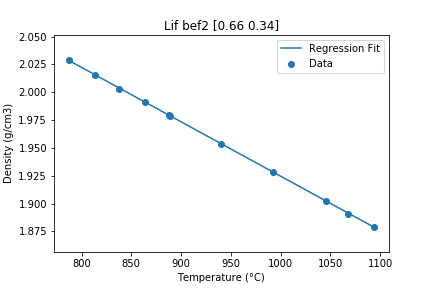
\includegraphics[width=\linewidth]{msdf/figures/lifbefBl.png}
\end{minipage}
\caption{Example output when asking for density analysis of $LiF-BeF_2$}
\label{fig:lifbef}
\end{figure}
\newpage